\documentclass{article}
\usepackage[utf8]{inputenc}
\usepackage{textcomp}
\usepackage{mathtools}
\usepackage{multirow}
\usepackage[tableposition=top]{caption}

\title{Improving IBD detection algorithms for genetic genealogy databases}
\author{Gregory R. Magoon\\Aerodyne Research, Inc.\\Billerica, Massachusetts, United States}
\date{September 2018}

\usepackage{natbib}
\usepackage{graphicx}

\begin{document}
\maketitle
\begin{center}
Copyright \copyright 2018 All Rights Reserved.
\end{center}

\begin{abstract}
    In recent years, with the proliferation of personal ancestry testing through microarray-based genotyping, detection of identity-by-descent (IBD) has become an important tool in genetic genealogy, enabling, for example, the identification and analysis of previously unknown biological relationships. The large amounts of data involved (hundreds of thousands to millions of individuals, and hundreds of thousands or more genotyped loci per individual) have prompted commercial databases and a prominent open, public database (GEDmatch) to adopt computationally streamlined approaches that are able to efficiently accommodate steadily incoming data, as new individuals are incorporated into the comparison databases. The tradeoff for computational efficiency with these approaches is a reduced ability to discriminate between IBD and non-IBD compared to more advanced approaches, especially when a) the two datasets being compared have limited density or limited overlap in genotyped loci, b) IBD segments of interest are small ($<\sim$7 cM) or c) genotypes have high error rates. Here, we consider several variations of these algorithms, and use Bayesian analysis to gain insight into the underlying statistics and develop improved algorithms. Of particular note, the analysis demonstrates the heretofore unappreciated importance of heterozygous-to-heterozygous situations that arise in the pairwise genotype comparisons. The results suggest several possible refinements to current approaches, and two specific possibilities are discussed and demonstrated with both simulated and real data. One approach involves a simple modification to the type of genotype comparisons that contribute to meeting locus count thresholds for candidate IBD segments. The second approach takes advantage of allele frequency knowledge to increase detection power, and incorporates a genotype error model to enable error tolerance in a tunable, statistically justified manner.
\end{abstract}

\section{Introduction}
Detection and analysis of identity-by-descent (IBD) between pairs of individuals or among cohorts of individuals has been the subject of extensive research, with wide-ranging applications across population genetics and medical genetics, including genome-wide association studies, or GWAS (e.g. \citep{GERMLINE} \citep{PLINK} \citep{Albrechtsen} \citep{beagle} \citep{speeDB} \citep{Parente2}  \citep{fastIBD} \citep{ERSA} \citep{ERSA2} \citep{decode}). A relatively recent, but powerful application of IBD detection is in the growing field of genetic genealogy.\citep{23andMe} Very recently, these new IBD-based genetic genealogy tools have also entered the field of forensic genetics.\citep{GSK}

The main IBD comparison databases include those of commercial ancestry testing services, such as 23andMe and AncestryDNA, as well as GEDmatch, a free and open database accepting raw genotyping data from the various ancestry testing services, enabling cross-company comparisons.\citep{GEDmatch}

Due to the extreme number of pairwise comparisons involved, and the need to run new pairwise comparisons as new samples continue to be added to a steadily growing comparison pool, these databases have adopted variations on a low-computational-cost IBD detection approach first described by Henn et al.\citep{23andMe} The algorithm involves looking for a contiguous set of genotyped markers lacking "opposite homozygotes" (i.e. AA vs. BB for a biallelic locus with possible symbolic alleles A and B). In addition to requiring that the set of markers span a minimal genetic distance (e.g. 7 cM), identifying a segment as IBD requires that the region lacking opposing homozygotes also span a minimum number of markers (e.g. 400 SNPs). This criterion helps to guard against detecting regions where the genotyped (but unphased) markers lack opposite homozygotes due to coincidental identity-by-state (IBS). The algorithm is elegant in its simplicity, compared to more advanced approaches, and it has apparently been independently implemented (with some variation in details, but sharing the same core framework) in at least four commercial databases (23andMe, AncestryDNA, My Heritage, and Family Tree DNA), as well as several third-party databases, including GEDmatch.

Although the algorithm's low computational cost and ease of implementation are very favorable features, it is not without limitations. Commenting on the algorithm described by Henn and colleagues, Huang et al. have noted that the algorithm lacks sensitivity compared to more advanced approaches (only reliably identifying segments larger than about 7 cM), and adopts an heuristic approach to account for sporadic genotype errors.\citep{speeDB} So the tradeoff for the simplicity of the algorithm is that it has limited ability to discriminate between IBD and non-IBD in more challenging use cases, such as when making comparisons between individuals genotyped on different microarray platforms, where there may be limited overlap between the two sets of genotyped markers. A similar sort of challenging use case arises when trying to use the algorithm with genotype sets derived from confident calls in low-coverage whole-genome sequencing (WGS) data. In such situations, a user must either accept a high rate of false negatives (due to the inability of genuine IBD segments to meet the marker count threshold), or reduce the marker count threshold (if given the option) in order to reduce false negatives, but with the side effect of increasing false positives related to IBS. 

Another issue is that expanding to broader marker sets (for example, arising from genotyping known variants based on WGS, tends to introduce a significant portion of loci with rare variants (allele frequencies close to zero or unity). As noted by Huang et al.,\citep{speeDB} these markers are usually not particularly informative in distinguishing IBD from non-IBD. The strong allele frequency bias associated with broader marker sets would be expected to lead to unreliable behavior in the algorithm as originally described by Henn and colleagues, at least without adjustments to the marker count threshold and the heuristics for handling genotyping error. One would want to incorporate allele frequency information into the algorithm, either indirectly (by excluding markers not meeting some minimum minor allele frequency threshold, for example) or directly (through, for example, a weighting approach as described later).

A key point worth noting in the context of this paper is that the different implementations of this algorithm have adopted a variety of approaches related to which genotype match situations they consider as counting towards meeting the marker count threshold (with the threshold correspondingly also varying in accordance with the inclusion or exclusion of certain genotype match situations). For a biallelic marker, in addition to the previously-discussed opposite homozygotes situation (inconsistent with half-IBD), three genotype match situations, all consistent with half-IBD, are possible: 1) matching homozygotes (e.g. AA vs. AA), 2) matching heterozygotes (AB vs. AB), and 3) one heterozygote vs. one homozygote (e.g. AB vs. AA). The approach described in the original paper of Henn and colleagues requires at least one of the two samples have a homozygous genotype in order for the locus to count towards the 400 SNP threshold, essentially excluding the second genotype match situation (het-to-het) from consideration. The original GEDmatch implementation considered all three types of genotype match situations in counting toward the SNP threshold (default of 500 SNPs for "one-to-one" pairwise comparisons). An implementation on GEDmatch's new "Genesis" platform only considers matching homozygotes, excluding the second and third genotype match situations (het-to-het and het-to-hom), while reducing the SNP threshold.

Here, we will use Bayesian statistical methods to argue that the most effective allele-frequency-agnostic approach involves considering the second genotype match situation (het-to-het) but excluding the third genotype match situation (het-to-hom), constituting a variation on the algorithm not used in any previous implementation at the time of this writing, to our knowledge. We will also demonstrate how consideration of allele-frequencies during match evaluation, wherein appropriate weighting factors are applied in the consideration of all three types of genotype match situations (in addition to the opposite homozygote mismatch situation), can lead to significant improvements in IBD vs. non-IBD discrimination power as well as improvements in accuracy of estimated IBD segment boundaries.

\section{Approach}
To analyze, with Bayesian statistical methods, the genotype match situations that can be considered within the framework of the IBD-detection algorithm of Henn and colleagues, we use the logarithm of likelihood ratios for half-IBD relative to non-IBD situations. These log likelihood ratios allow the contribution of each locus comparison to be considered independently and in an additive manner. The summation of these log likelihood ratios might be considered to provide an indication of the likelihood of a given region being half-IBD rather than non-IBD. Thus, the summed log likelihoods might be considered as serving the same purpose as the marker threshold in the algorithm of Henn and colleagues, representing an aggregate body of evidence to rule out coincidental IBS. A similar log likelihood approach was adopted in the development of the Parente2 algorithm, but considered likelihoods for haplotypes rather than genotypes.\citep{Parente2} The ratios are derived as a function of each locus' (possibly unknown) allele frequency and the specific genotype match situation arising in a particular pairwise match at that locus.

For the purposes of this paper, we restrict the scope to considering detection of half-IBD only, without considering the possibility of full-IBD. Full-IBD will typically only be seen in close (e.g. sibling) relationships or in cases where the parents of the individuals being compared are from the same endogamous population. And, in any case, full-IBD situations will generally be identified by half-IBD detection algorithms.

We also restrict to consideration of loci recognized as biallelic, for the sake of simplicity. These loci will typically be single-nucleotide polymorphisms (SNPs) in applications of the algorithms discussed, but this need not necessarily be the case, and small insertions or deletions (indels) might also be considered, for example.

\subsection{Simple refined approach}
To gain insight into the statistics underlying the genotype comparisons used in the algorithm of Henn and colleagues, we initially consider likelihood ratios based on a simple allele frequency model, without accounting for the possibility of genotyping error or \textit{de novo} mutation. The log likelihood ratios, $\ln K_i$, for marker $i$, consider the ratio of the probability of observing a given genotype combination, $G_{mn,i}$ between individuals $m$ and $n$, given that the marker is within an IBD segment, to the probability of observing the same genotype combination given that the marker is not within an IBD segment, as follows:
\begin{equation}
  \ln K_i = \frac{P(G_{mn,i} | \text{half-IBD})}{P(G_{mn,i} | \text{non-IBD})}
\end{equation}
The allele-frequency-dependent probabilities considered here are equivalent to those presented in Table 1 of Epstein et al.,\citep{RELPAIR} except that we consider order-agnostic genotype combinations rather than ordered genotype pairs, and also restrict to a biallelic model. Although we model allele frequencies here for purposes of analysis, we consider the allele frequencies to be unknown, in this section, for purposes of developing a refined algorithm. This corresponds to the situation with the algorithm of Henn and colleagues, where allele frequencies are not taken into consideration.

In the following figure, we plot the log likelihood ratios for the three matching genotype situations (plus two additional situations with the A and B alleles swapped) as a function of the allele frequency of the B allele. In the figure, positive values correspond to a likelihood ratio favoring IBD, while negative values favor non-IBD. The curves for the situations with the A and B alleles swapped are simply the reflection of the curve for the original situation about $x_{B,i}=\frac{1}{2}$ where $x_{B,i}$ is the B allele frequency.

\begin{figure}[h!]
\noindent
\centering
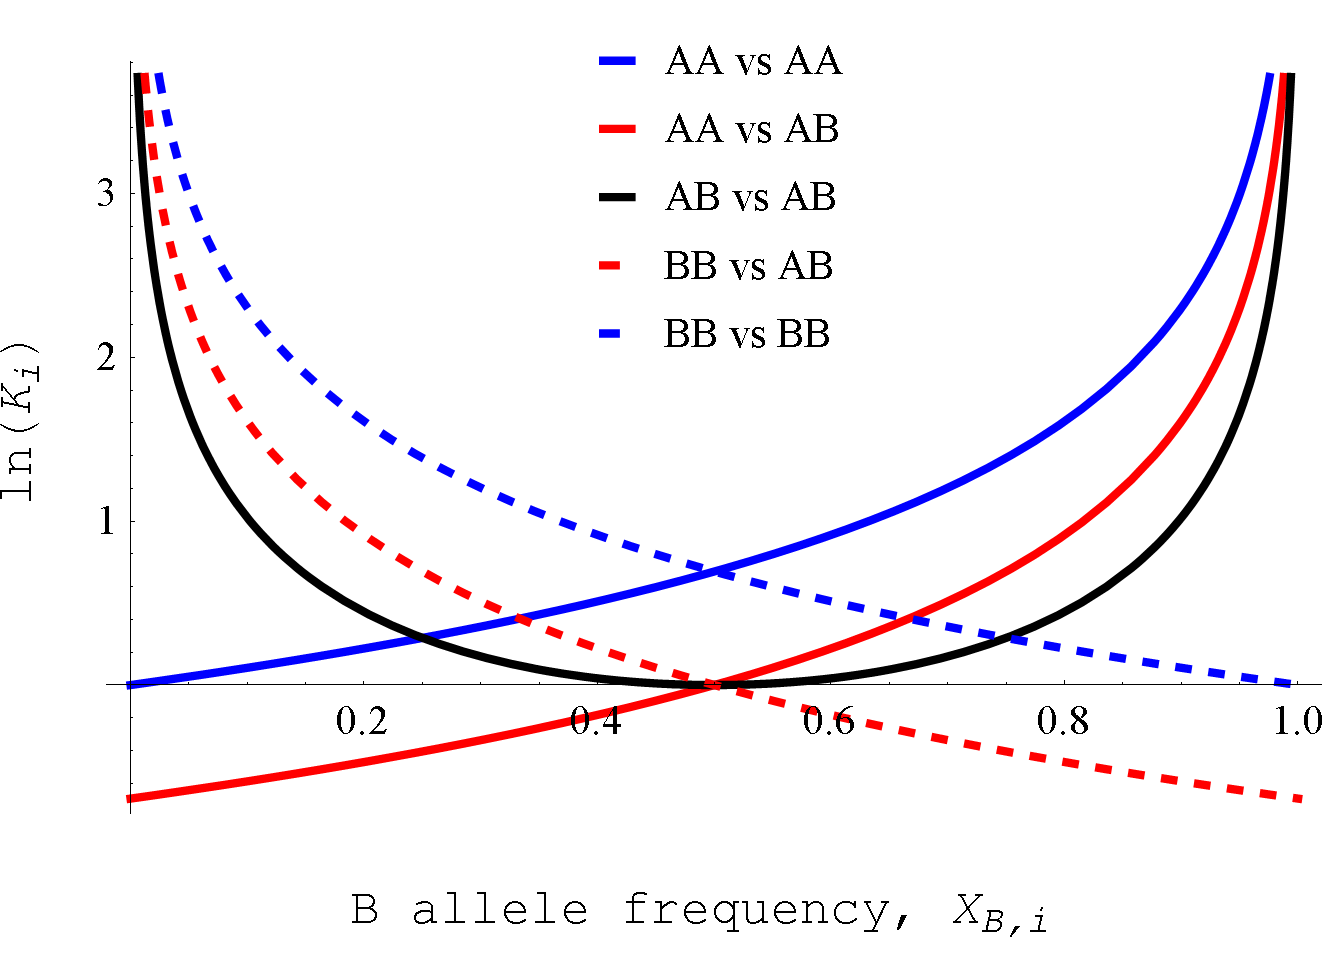
\includegraphics[scale=0.20]{llrs_rev2c}
\caption{Log likelihood ratios for half-IBD relative to non-IBD in various matching genotype situations.}
\label{fig:llrs}
\end{figure}

From the figure, it can be seen that the observed genotype situations favor IBD in most cases, with a few exceptions. The log likelihood ratios for the het-to-het and hom-to-het situations are zero with allele frequencies of $\frac{1}{2}$, indicating that these observations, at a marker with equal allele frequencies, do not provide any IBD-relevant information in the context of the algorithm. Similarly, the hom-to-hom situation also provides no new information when the observed allele has frequency of unity. Next, and perhaps contrary to what one might intuitively expect, the hom-to-het situation has negative log likelihood ratio when the frequency of the shared allele (i.e. B in BB vs. AB) is above $\frac{1}{2}$, indicating that this observation is actually suggestive of non-IBD. In contrast, it can be seen that the het-to-het situation is strongly suggestive of IBD when one of the alleles is rare.

The log likelihood curve for the hom-to-het situation deserves further discussion. As noted previously, when the shared allele has frequency above $\frac{1}{2}$, the log likelihood ratio is slightly negative, suggestive of non-IBD rather than IBD. The log likelihood ratio passes through zero for allele frequencies of $\frac{1}{2}$, and becomes positive when the shared allele has frequency below $\frac{1}{2}$. Now, we expect that most of the times a hom-to-het situation is observed will involve sharing of the more common allele, suggesting that the negative portion of the curve may dominate in practice. 

Indeed, with certain assumptions on the anticipated allele frequencies, we can calculate expectation values for the log likelihood ratios for each genotype match situation. These expectation values provide an indication of the IBD-relevant information each type of genotype match situation can provide in an allele-frequency-agnostic detection algorithm in the framework of the approach described by Henn and colleagues.

Here, we derive allele frequency probability distributions for each genotype match situation by first assuming a uniform, Beta(1,1) prior on the B allele frequency, $X_{B,i}$. Then, we incorporate information from the observed allele counts in the two samples (assuming either half-IBD or non-IBD situations) to derive a posterior probability distribution for the B allele frequency. Since the conjugate prior to the binomial genotype combination probability model is a beta distribution, this posterior distribution is also a beta distribution.

The resulting allele frequency probability distributions then allow us to compute the integrals needed to determine the expectation value for the log likelihood ratio for each genotype match situation. The results are shown in the following table, assuming either half-IBD or non-IBD scenarios. For each scenario, the table indicates the modeled probability distribution for the B allele frequency, as well as the corresponding expectation value for the log likelihood ratio.

\begin{table}[h]
\caption{Expectation value of log likelihood ratios, with uniform prior on B allele frequency, $X_{B,i}$}
\label{tab:expectationvalue}
\centering
\noindent
\begin{tabular}{ |c|c|c|c|c|c| }
\hline
\multicolumn{2}{ |c| }{Genotype match} & \multicolumn{2}{ |c| }{assuming non-IBD} & \multicolumn{2}{ |c| }{assuming half-IBD}\\\hline
Type & Alleles & $X_{B,i}$ & $E[\ln K_i]$ & $X_{B,i}$ & $E[\ln K_i]$ \\\hline
\multirow{2}{*}{hom-to-hom} & AA vs. AA & Beta(1,5) &  \multirow{2}{*}{0.20} & Beta(1,4) & \multirow{2}{*}{0.25}\\
 & BB vs. BB & Beta(5,5) & & Beta(4,4) &  \\\hline
het-to-het & AB vs. AB & Beta(3,5) & 0.18 & \parbox[c]{2 cm}{$\frac{1}{2}$ (Beta(2,4) \\ + Beta(3,4))} & 0.28 \\\hline
\multirow{2}{*}{hom-to-het} & AA vs. AB & Beta(2,5) &  \multirow{2}{*}{-0.24} & Beta(2,4) & \multirow{2}{*}{-0.11}\\
 & BB vs. AB & Beta(4,5) & & Beta(3,4) &  \\
\hline
\end{tabular}
\end{table}

We see from the table that the expected log likelihood ratio, under the given assumptions, for the het-to-het and hom-to-hom situations are positive and similar in magnitude. Furthermore, most marker sets would be expected to follow an allele frequency spectrum more strongly biased towards zero and unity than the uniform prior considered here. Adopting a more rare-variant biased prior would further increase expectation value for the het-to-het log likelihood ratio while reducing that for the hom-to-hom situation.

The expected log likelihood ratio for the hom-to-het situation is negative and comparable in magnitude to the positive het-to-het and hom-to-hom values.

Taken together, this suggests a variation on the algorithm of Henn and colleagues, wherein hom-to-hom and het-to-het situations are considered to count towards meeting the marker count threshold (appropriately adjusted to achieve favorable balance between false negatives and false positives), while hom-to-het situations are ignored. Indeed, the negative expectation value for hom-to-het log likelihood ratio might argue for actually subtracting from the marker count when these genotype match situations are encountered. On the other hand, the log likelihood ratio for hom-to-het genotype match situations is not universally negative, and can actually be strongly suggestive of IBD when the shared allele is rare. This naturally leads to a second, more advanced refinement to the algorithm, discussed in the next section, wherein knowledge of allele frequencies is taken into consideration.

\subsection{Allele-frequency-aware, error-rate-aware refined approach}
We also incorporate a genotype error model, similar to the approach used in speeDB.\citep{speeDB}
[to be added]

\section{Results}
\subsection{Refined algorithm performance tests}
[to be added]

\section{Conclusion}
We have demonstrated here the importance of heterozygous-to-heterozygous situations in variations on the IBD detection algorithm of Henn et al. [to be added] 

\section{Disclosure}
Through his employer, G.R.M. works with Full Genomes Corporation (Harrisonburg, VA), a company utilizing massively parallel / "next-generation" sequencing in the fields of consumer genomics, genetic genealogy, and forensic genetics.
...

\bibliographystyle{unsrt}
\bibliography{references}
\end{document}
